\documentclass[11pt]{report}
\usepackage[T1]{fontenc}
% \usepackage [latin1]{inputenc}
\usepackage{fontawesome} %icons

% Images
\usepackage{graphicx}
\usepackage{float}
\usepackage{caption}
\usepackage{subcaption}

% Links
\usepackage[hidelinks]{hyperref}

% References
\usepackage{csquotes}
\usepackage[spanish,activeacute]{babel}
\usepackage[
    backend=biber,
    sorting=none,
    citestyle=numeric,
    bibstyle=science
]{biblatex}
\addbibresource{references.bib}

% Avoid indenting each line
\setlength{\parindent}{0pt}

% Custom colors
\usepackage[dvipsnames]{xcolor}
	\definecolor{white}{RGB}{255,255,255}
	
% Blocks of code
\usepackage{listings}
  \definecolor{codegreen}{rgb}{0,0.6,0}
  \definecolor{codegray}{rgb}{0.5,0.5,0.5}
  \definecolor{codepurple}{rgb}{0.58,0,0.82}
  \definecolor{backcolour}{rgb}{0.95,0.95,0.92}

  \lstdefinestyle{mystyle}{
     backgroundcolor=\color{backcolour},   
     commentstyle=\color{codegreen},
     keywordstyle=\color{magenta},
     numberstyle=\tiny\color{codegray},
     stringstyle=\color{codepurple},
     basicstyle=\ttfamily\footnotesize,
     breakatwhitespace=false,         
     breaklines=true,                 
     captionpos=b,                    
     keepspaces=true,                 
     numbers=none,                    
     numbersep=5pt,                  
     showspaces=false,                
     showstringspaces=false,
     showtabs=false,                  
     tabsize=2
  }
  \lstset{style=mystyle}

% - Front page
\usepackage{tikzpagenodes}
\usepackage{ragged2e}
  \addto\captionsspanish{\renewcommand{\contentsname}{Índice}}

% Page format
\usepackage[margin=2cm, top=2cm, includefoot]{geometry}
  \addtolength{\topmargin}{-1cm}
\usepackage{fancyhdr}
  \renewcommand{\chaptermark}[1]{\markboth{#1}{}}
  \setlength{\headheight}{80pt}
  \pagestyle{fancy}
  \fancyhf{}
  \fancyfoot[C]{\thepage}
  \lhead{
    \hyperref[chapter:contents]{
\includegraphics[height=40pt]{images/UPCT-header.png}}
    \ifnum\value{chapter}=0 {}
    \else {{\hfill \Large \thechapter\ \itshape $\vert$ \leftmark \hspace{5cm} \hfill}}
    \fi
} 
% \rhead{\includegraphics[height=35pt]{image.png}}
\renewcommand{\headrulewidth}{3pt}
\renewcommand{\headrule}{\hbox to\headwidth{\color{RoyalBlue}\leaders\hrule height \headrulewidth\hfill}}

% Chapter format
\usepackage{chngcntr}
	\counterwithout{figure}{chapter}
	\counterwithout{table}{chapter}
\usepackage{etoolbox}
\usepackage[Glenn]{fncychap}
  \addto\captionsspanish{\renewcommand{\chaptername}{Sección}}
\makeatletter
\patchcmd{\@makechapterhead}{\vspace*{50\p@}}{\vspace*{-20\p@}}{}{}
\patchcmd{\@makeschapterhead}{\vspace*{50\p@}}{\vspace*{-20\p@}}{}{}
\patchcmd{\DOTI}{\vskip 80\p@}{\vskip 40\p@}{}{}
\patchcmd{\DOTIS}{\vskip 40\p@}{\vskip 0\p@}{}{}
\makeatother

% -- Custom functions
% CLI
\usepackage{soul}
	\sethlcolor{black}
\newcommand{\cli}[1]{%
  \mbox{%
		\textcolor{white}{\hl{#1}}%
  }%
}

% Inline code
\usepackage{tikz}
\newcommand{\icode}[1]{%
  \raisebox{-.1cm}{%
    \begin{tikzpicture}%
      \node[rectangle, rounded corners, fill=black!30]{#1};%
    \end{tikzpicture}%
  }%
}

% Code block
\newcommand{\code}[2]{%
  \lstinputlisting[language=#2]{snippets/#1}%
}

% Image
\newcommand{\credit}[1]{%
  \begin{flushright}%
    \item #1%
  \end{flushright}%
}

\newcommand{\image}[3]{%location, width, caption
  \begin{figure}[H]%
    \centering%
    \includegraphics[width=#2]{images/#1}%
    \caption{#3}%
  \end{figure}%
}

% File
\newcommand{\lined}[1]{\smash{\begin{tabular}{l} \hline #1 \\ \hline \end{tabular}\hspace*{-\tabcolsep}}} %lined 
\newcommand{\file}[3]{%location, name, lang
  \par%
  \lined{%
    \textbf{%
      \faCode \ \color{gray}{\texttt{#1/#2}}%file path
    }%
  }%
  \vspace{-.1cm}%
  \code{#2}{#3}%file content
}


\begin{document}
  \begin{titlepage}   
    \begin{tikzpicture}[remember picture,overlay,shift={(current page.north west)}]
		\node[anchor=north west, xshift=-.2cm,yshift=.2cm]{
\includegraphics[height=\paperheight]{images/UPCT-sidebar.png}};
	\end{tikzpicture}
    
    \vspace{5cm}
    {\centering
        \hspace{3cm}
\includegraphics[width=.7\textwidth]{images/UPCT-front.jpg}
        
        \vspace{5cm}
        \hspace{2cm}\huge\textbf{\color{RoyalBlue}Desarrollo de un teclado para el S.XXI, accesible y con MicroPython} 
        
        {\LARGE
        \vspace*{\fill}
        \begin{flushright}
          \item Autor: Pablo Martínez Bernal
          \item Director: Jose Alfonso % !!
          \item Máster Universitario en Ingeniería de Telecomunicación
          \item \textit{Curso 2022-23}   
        \end{flushright}
        }
    }
\end{titlepage}


  % {\null\thispagestyle{empty}\newpage}

  \chapter*{Resumen}
    En la actualidad es cada vez más la gente que pasa varias horas al día delante de un ordenador, nuestra principal herramienta para controlarlos es el teclado y, sin embargo, su diseño apenas ha avanzado desde su aparición. Este diseño arcaico supone problemas de salud, falta de accesibilidad y reduce la productividad. \vspace{0.3cm} \par

Por esto, en el presente documento se estudian los avances y variaciones que ha realizado la comunidad de aficionados en los últimos años y se detalla el diseño y construcción de un teclado más acorde al mundo actual que solventa los problemas recién citados, así como permitiendo una gran capacidad de personalización gracias a su diseño hardware que permite cambiar componentes fácilmente y el desarrollo de un firmware y software \textit{open source} fácilmente editables.



  \chapter*{Lista de acrónimos usados}
    \textbf{HID} Human Device Interface - Protocolo de comunicación sobre USB
\textbf{I2C} Inter Integrated Circuit - Protocolo de comunicación entre circuitos integrados
\textbf{MCU} Micro Controller Unit
\textbf{PCB} Printed Circuit Board
\textbf{SPI} Serial Peripheral Interface - Protocolo de comunicación entre circuitos integrados


  \tableofcontents \label{chapter:contents}


  \chapter{Introducción}
    \section{Motivación}
Hoy en día, es mucha la gente que se pasa buena parte del día frente a un ordenador, tanto por trabajo como en su tiempo libre. Esto, por supuesto, puede suponer problemas para la salud si no se toman las precauciones necesarias. Por ejemplo, problemas de vista por pasar excesivas horas mirando un monitor, aunque en este frente ya hay una buena cantidad de divulgación e investigación.

Sin embargo, el periférico que más usamos es el teclado y, sin embargo, su \emph{problemático} diseño apenas ha cambiado desde que existen los ordenadores y puede resultar en diversas lesiones y enfermedades en las muñecas.

\section{Objetivo}
El principal fin de este trabajo va a ser el diseño de un teclado que se adapte mejor a la anatomía humana y que, a su vez, incorpore mejoras que lo hagan accesible a gente con diversas discapacidades:
\begin{itemize}
  \item Teclas con letras grandes y alto contraste
  \item Un joystick integrado que permita controlar el teclado
  \item Solenoide para mayor feedback táctil y sonoro
\end{itemize}

    

  \chapter{Preámbulo}
    \section{Requisitos previos}
En la siguiente sección, se asume que ya tenemos \mycite{git}, \mycite{python} y \mycite{vscode} instalados. En el editor podemos ir instalando distintas extensiones para autocompletado de sintaxis en lenguajes que no estén soportados de base y herramientas de ayuda. Estos complementos no son \textit{necesarios} y su instalación es tan trivial como ir al apartado de \myemph{extensiones}, por lo que no comentaré nada sobre ellos.

\section{Configuración para trabajar en remoto}
El desarrollo de este trabajo ha sido realizado en una máquina Arch Linux, controlada por SSH desde Windows, por lo que en el informe se verán comandos, imágenes y archivos que mezclan ambos sistemas operativos. Salvo que se especifique lo contrario, cualquier adjunto pertenece a Linux. \par
\myemph{Nota}: En otras distribuciones de Linux, habría que usar otros gestores de paquetes, como \cli{apt-get} o \cli{zypper} y es posible que algun programa esté empaquetado con un nombre distinto.

  \subsection{SSH}
  Para poder trabajar cómodamente en la terminal, generamos una clave SSH en windows con \cli{ssh-keygen} y la salida del comando se guarda en \icode{C:/Users/<usuario>/.ssh/id\_<encriptado>.pub} \newline
  El contenido de este archivo lo copiamos en Linux en \icode{$\sim$/.ssh/authorized\_keys}, gracias a esto podremos conectarnos en remoto a Linux sin necesidad de introducir las credenciales, puesto que hemos añadido la identidad de la máquina Windows como un dispositivo de confianza.

  \subsection{Montar disco en red}
  Con el fin de acceder de forma cómoda y rápida a los archivos Linux, en vez de estar usando SCP o SSH he montado una ubicación de red en Windows. Instalamos con \cli{sudo pacman -S samba} y activamos los servicios \cli{sudo systemctl enable smb} y \cli{sudo systemctl enable nmb}. Tras crear el usuario e introducir en Windows las credenciales, tenemos acceso a todo el \icode{\$HOME} de nuestro Linux:
  \image{linux-home}{.6\textwidth}{Carpeta montada en Windows}

  \subsection{git}
  Al intentar usar la carpeta recién montada, surge un problema puesto que la instalación de git no confía en el repositorio, para arreglar esto debemos ejecutar \newline
  \cli{git config --global --add safe.directory '%(prefix)///192.168.1.200/elpekenin/Coding/access_kb'}

  \subsection{Servidor X}
  Para poder desarrollar el programa en Linux y testearlo desde Windows, debemos instalar un servidor que nos proporcione compatibilidad con la interfaz gráfica de Linux, he usado \mycite{vcxsrv}. A partir de ahora cuando nos conectemos a la máquina de desarrollo, añadimos la opcion \icode{-X} al comando SSH, para habilitar el redireccionamiento de los gráficos(por defecto está activa, pero prefiero añadirla por si acaso)

  \subsection{\LaTeX}
  Este informe lo he escrito en \LaTeX, instalamos el software necesario con \cli{sudo pacman -S texlive-most} \newline
  Para poder ver la salida PDF, he instalado un visor minimalista \cli{sudo pacman -S mupdf} y como el compilado de \LaTeX incluye varios pasos, he añadido una función a mi configuracion de shell (uso ZSH)
  \code{$\sim$}{.zshrc}
  Este comando se ejecuta haciendo simplemente \cli{pdf}. Funciona de forma silenciosa, redirigiendo la salida de los comandos para que no salgan por pantalla; y al terminar abre el archivo producido.
  \image{pdf-view}{.5\textwidth}{Viendo el PDF en Windows}


  \chapter{Estado del arte}
    \section{Diseño}
      \begin{figure}[H]
  \begin{subfigure}[b]{.5\textwidth}
    \centering
    \includegraphics[width=.8\textwidth]{images/model\_m}
    \caption{Teclado IBM Model M (1984)}
  \end{subfigure} 
  \hfill
  \begin{subfigure}[b]{.5\textwidth}
    \centering
    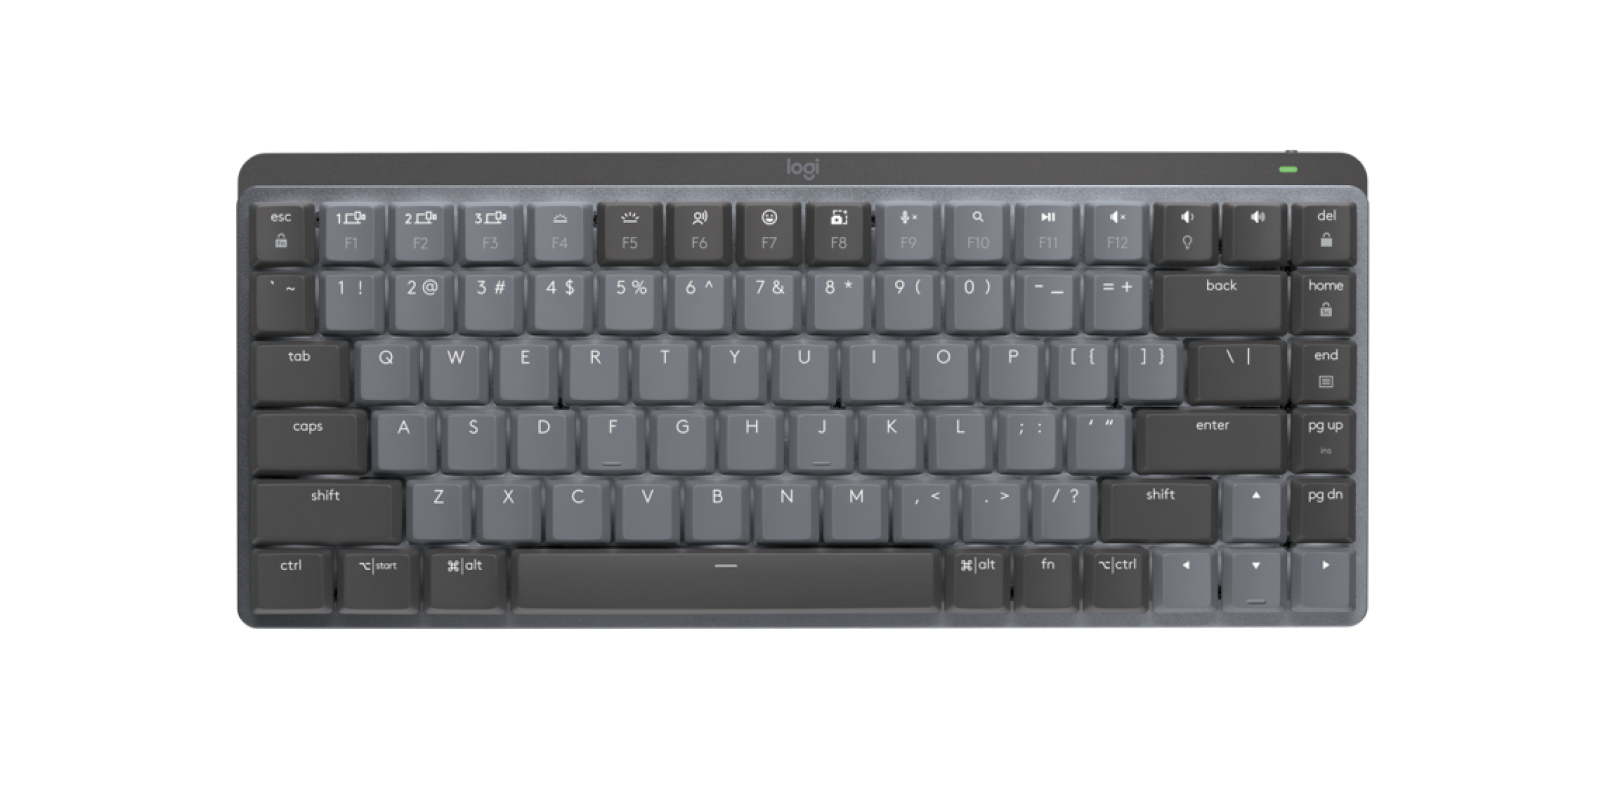
\includegraphics[width=\textwidth]{images/logitech}
    \caption{Teclado Logitech MX Mechanical (2022)}
  \end{subfigure}
  \caption{Comparativa teclado antiguo y actual}
\end{figure}

\image{android\_keyboard}{.4\textwidth}{Teclado en Android}

Como podemos ver, los teclados no han variado en los ultimos 40 años, ni siquiera para adaptarse a las pequeñas pantallas táctiles de los móviles.

\subsection{Diseño anticuado}
  \subsubsection{Forma del teclado}
  Quizás nunca nos lo hayamos preguntado puesto que tenemos muy interiorizada la forma de los teclados, pero si lo pensamos un poco, es peculiar la posición relativa de las teclas. Cada fila tiene un pequeño desfase con las demás en vez de estar alineadas. Esto es un legado de sus antecesoras, las máquinas de escribir, donde por limitaciones mecánicas esto tenía que ser así y evitar choques entres las piezas móviles de cada tecla.
  \image{typewriter}{.3\textwidth}{Detalle de las letras en una máquina de escribir}

  Este posicionamiento relativo de las teclas supone un problema a la hora de escribir, ya que la forma óptima de hacerlo sería la siguiente:
  \image{mechanography}{.3\textwidth}{``Mapa'' de mecanografía}
  
  Sin embargo, para escribir así, las muñecas terminan en posiciones un poco forzadas, y los dedos hacen movimientos incómodos. Para arreglar esto surgieron los teclados ortolineales, donde todas las filas están alineadas y los dedos se mueven en una línea recta. Estos teclados suelen tener todas las teclas del mismo tamaño, optimizando así la cantidad de teclas que podemos tener ocupando el mismo espacio (donde antes había una barra espaciadora pueden entrar varias teclas). Como se puede ver en la siguiente imagen, normalmente también prescinden del teclado numérico para reducir el tamaño, este modelo se conoce como ``75\%'' ya que tiene 75 teclas mientras que los teclados comunes (``100\%'') tienen 104/105 teclas. Otras variantes comunes son ``40\%'', ``60\%'', ``65\%'' 
  \image{ortholinear}{.3\textwidth}{Teclado ortolineal \textit{RGB75}}

  \subsubsection{Ubicación de las letras}
  Otro legado que nos dejaron las máquinas de escribir es la distribución QWERTY, que probablemente sea la única distribución que hemos visto a lo largo de nuestra vida. El problema con esta disposición es que, si bien distribuye las letras de forma que se usan las dos manos por igual, se diseñó en la decada de 1860, por lo que uno de sus objetivos era el de reducir los atascos en las máquinas de escribir separando las teclas más usadas de la parte central. 

  En contra, ahora que gracias a la electrónica no tenemos estas limitaciones, se han diseñado distribuciones que minimizan la distancia media que se debe recorrer al escribir, por lo que una vez acostumbrados a ellas se puede escribir más rápido y reduciendo la fatiga en los dedos. Las dos más extendidas son DVORAK y COLEMAK. 
  \image{qwerty}{.3\textwidth}{Distribución QWERTY}
  \begin{figure}[H]
    \begin{subfigure}[b]{.5\textwidth}
      \centering
      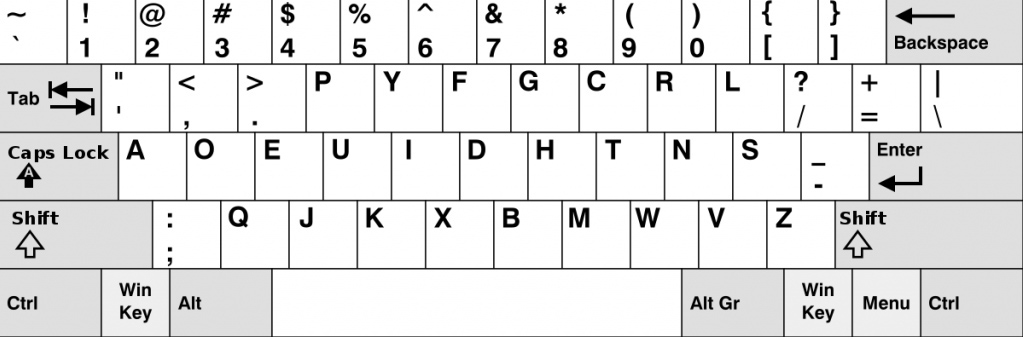
\includegraphics[width=.6\textwidth]{images/dvorak}
      \caption{Dvorak}
    \end{subfigure} 
    \hfill
    \begin{subfigure}[b]{.5\textwidth}
      \centering
      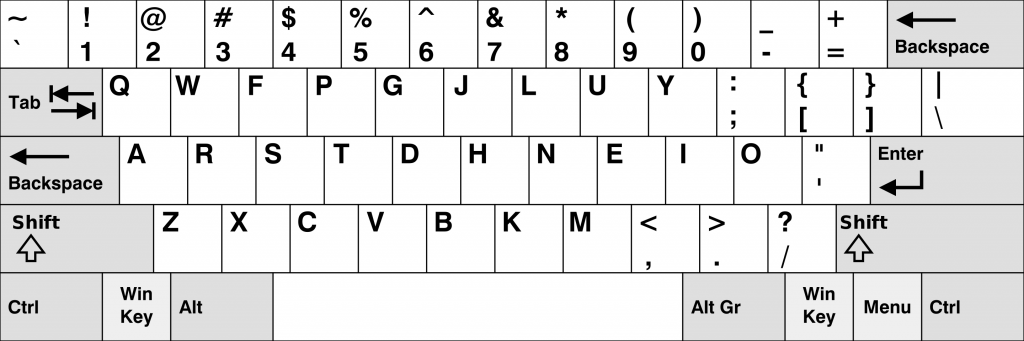
\includegraphics[width=.6\textwidth]{images/colemak}
      \caption{Colemak}
    \end{subfigure}
    \caption{Distribuciones alternativas}
  \end{figure}

\subsection{Algunos avances}
Gracias a la apasionada y extensa comunidad de aficionados a los teclados mecánicos, en los últimos años han aparecido multitud de diseños que incorporan diferentes cambios respecto al paradigma actual, algunos de estos conceptos son:
  \subsubsection{\textit{Split}}
  Como hemos comentado ya, uno de los problemas más comunes en gente que usa mucho los teclados es la aparicion de dolencias en las muñecas, a fin de que estas se posicionen de una forma más natural y cómoda, se opta por partir el teclado en dos mitades.
  \image{quefrency}{.5\textwidth}{Teclado \textit{Quefrency}}

  \subsubsection{Pulgares}
  Muchos teclados dotan de una mayor utilidad a los pulgares, que normalmente solo utilizamos para la barra espaciadora, añadiendo unas cuantas teclas en lo que comunmente se conoce como \textit{thumb cluster}.
  \image{ergodox}{.4\textwidth}{Teclado \textit{Ergodox}}

  \subsubsection{Reposamuñecas}
  Otros diseñadores aprovechan la oportunidad para integrar este accesorio de una forma más eficaz que la típica ``rampa'' de plástico que estamos acostumbrados a ver.
  \image{moonlander}{.4\textwidth}{Teclado \textit{Moonlander}}

  \subsubsection{\textit{Tenting}}
  Esta conocida técnica solo se puede aplicar en teclados \textit{split} y consiste en levantar la parte central del teclado, de forma que la muñeca está en una posición más natural en vez de estar paralela al plano que genera la mesa. Lo mejor de esta mejora es que se puede añadir a cualquier teclado que no la incorpore en sudiseño añadiendo algún objeto para levantarlo.
  \image{dygma}{.4\textwidth}{Teclado \textit{Dygma Raise}}

  \subsubsection{Ergonomía}
  El mayor ejemplo de esta filosofía de diseño es el \textit{Dactyl Manuform}, un teclado que debido a su particular forma ni siquiera puede funcionar con una PCB (placa de circuito impreso) y tiene que soldarse a mano la unión entre todos sus componentes. El beneficio de su diseño es que tiene en cuenta la forma de las manos, por lo que las teclas se encuentra posicionadas acorde al movimiento de los dedos. Además, hay usuarios que optan por modificar el diseño e integrarle una \textit{trackball} para poder controlar el cursor sin tener que mover la mano entre el teclado y el ratón.
  \image{manuform}{.5\textwidth}{Teclado \textit{Dactyl Manuform} con trackball}

      \newpage

    \section{Hardware}
      \subsection{Cableado de las teclas}\label{sec:scanning}
    \subsubsection{Conexión directa}
    La opción más sencilla que se nos puede ocurrir para conectar diversos interruptores a nuestro microcontrolador es soldarlos directamente a los pines de entrada/salida(GPIO). Para hacer esto tenemos 2 opciones:
    \begin{figure}[H]
        \begin{subfigure}[b]{.5\textwidth}
          \centering
          \includegraphics[width=.5\textwidth]{images/pull\_down}
          \caption{Pulsador con resistencia Pull-Down}
        \end{subfigure} 
        \hfill
        \begin{subfigure}[b]{.5\textwidth}
          \centering
          \includegraphics[width=.5\textwidth]{images/pull\_up}
          \caption{Pulsador con resistencia Pull-Up}
        \end{subfigure}
        \caption{Cableado directo}
      \end{figure}
    
    Si hacemos esto, sin embargo, tendremos un problema pronto porque necesitaremos un chip con muchos pines de entrada/salida, o hacer un teclado con pocas teclas porque la cantidad de GPIOs es reducida.

    \subsubsection{Matriz}
    Para solventar este problema, podemos cablear los botones mediante una matriz, usando un pin para cada fila y columna de teclas. Usamos una dimensión como salida y otra como entrada, haciendo un bucle que aplique voltaje en cada una de las filas y compruebe si las columnas reciben una entrada (tecla pulsada cerrando el circuito). \emph{Nota: También se podría iterar en la otra dimensión}
    \image{matrix}{.2\textwidth}{Cableado en matriz}

    Este diseño también tiene sus problemas, el más notorio es el conocido como ``efecto \textit{ghosting}'' en el que podemos detectar como pulsada una tecla que no lo está.
    \image{ghosting}{.2\textwidth}{Ghosting en una matriz}

    En este ejemplo, la tecla \textbf{(1, 1)} se detecta como pulsada de manera correcta pero, al pulsar también las teclas \textbf{(0, 1)} y \textbf{(0, 0)}, estamos cerrando el circuito y generando que en la columna 1 llegue voltaje a la entrada, que será interpretado como que la tecla \textbf{(1, 0)} ha sido pulsada puesto que estamos en la iteración de la fila 0.\vspace{0.2cm}\par

    Este problema se solventa de forma sencilla, añadiendo unos diodos que bloqueen esta retroalimentación permitiendo detectar \textbf{(1, 1)} pero sin la pulsación falsa de \textbf{(1, 0)} del caso anterior.
    \image{anti\_ghosting}{.3\textwidth}{Matriz anti-ghosting}

    Aunque no es muy grave, para matrices muy desiguales, por ejemplo 5x20 teclas, no estamos usando eficazmente los pines, ya que para esas 100 teclas estamos empleando 25 pines mientras que una configuración 10x10(20 pines) sería suficiente. \newline
    En este caso, podriamos hacer una distribución de teclas en forma rectangular, pero luego cablearlas como dicha matrix cuadrada, sin embargo el diseño sería bastante más confuso. \par

    Por último hay que tener en cuenta que, aunque el uso de los pines sea más óptimo, seguimos necesitando una cantidad de pines cada vez mayor conforme queramos añadir más teclas, aunque esto no debería ser un factor limitante en la mayoría de casos ya que este límite seguiría permitiendo una cantidad bastante elevada de teclas.

    \subsubsection{Lectura en serie}
    La opción que vamos a usar, inspirada en el \textit{ghoul}\cite{ghoul}, consiste en el uso de registros de desplazamiento conectados en una \textit{daisy chain}, de esta forma vamos a emplear un único pin para leer todas las teclas en una señal serie, y otros pocos pines (unos 3 o 4) para controlar estos chips mediante SPI\cite{spi} o I2C\cite{i2c}. De esta forma, podemos escanear potencialmente cualquier cantidad de teclas sin aumentar el números de pines necesarios, simplemente añadimos más registros a la cadena (aunque el escaneo se iría haciendo más y más lento)

\subsection{Pantallas}
En los últimos años es cada vez más común ver teclados que incorporan pequeñas pantallas, sin embargo, no son muy útiles ya que en la gran mayoría de casos se trata de SH1106 o SSD1306, que son dispositivos OLED de 2 colores y con una resolución bastante reducida, de 128x32 o 128x64 píxeles, en torno a la pulgada de diagonal. En nuestro teclado vamos a usar pantallas más potentes para poder mostrar información útil en vez de pequeños dibujos en estas pantallas más comunes.

\subsection{Sensor táctil}
También es relativamente común encontrar diseños que incluyen diferentes sensores (por ejemplo joysticks analógicos o PMW3360) para mover el sensor por la pantalla del ordenador sin tener que mover la mano hasta el ratón. Tal como podemos ver en el dactyl (\ref{img:dactyl}) \par 
En nuestro caso, puesto que vamos a añadir una pantalla, podemos aprovechar y usar una táctil, de forma que nos sirva para mover el cursor pero tambíen para tener una pequeña interfaz de usuario en el teclado.
      \newpage

    \section{Firmware}
      \subsection{Funcionalidad}
La mejor parte de usar una librería tan extendida como lo es QMK es que tenemos muchas facilidades a la hora de escribir el codigo ya que buena parte del trabajo está hecho ya. Esto incluye
\begin{itemize}
    \item Gestión sobre USB para reportar distintos endpoints (teclado, ratón, multimedia)
    \item Drivers para diversos periféricos tales como las pantallas ya comentadas, piezoelectricos para tener feedback sonoro o solenoides para vibración al pulsar las teclas, por nombrar algunos...
    \item Abstracciones para poder usar la misma API en diversos microcontroladores que internamente utilizan código y hardware muy diferente
    \item Documentación extensa y detallada
    \item Servidor ofcial en Discord donde podemos encontrar ayuda
\end{itemize}

\subsection{Escaneo de teclas}
Como se ha comentado en el apartado anterior, vamos a usar registros de desplazamiento, sin embargo QMK tiene soporte para cableado directo, en matrices y usando algunos otros circuitos, como \textit{IO expanders}. Sin embargo este no es el caso para los registros por lo que tendemos que escribir un poco de código para leer su información.

\subsection{Pantallas}
QMK tiene una API estandarizada (Quantum Painter\cite{qp}) para primitivas de dibujo en interfaces gráficas. Aún es ``joven'' y no soporta demasiadas pantallas, pero hace gran parte del trabajo por nosotros.

\subsection{Pantalla táctil}
QMK también tiene una capa de abstracción\cite{pointing} para diversos sensores que permiten mover el cursor, sin embargo todos se basan en medir desplazamientos y no una coordenada como es el caso de la pantalla táctil, por tanto en este caso nos vemos obligados a diseñar una arquitectura de software nueva, para poder trabajar con este otro tipo de datos de entrada.



  \chapter{Desarrollo}
    \section{Hardware}
      \section{Cableado de las teclas}
    \subsection{Conexión directa}
    La opción más sencilla que se nos puede ocurrir para conectar diversos interruptores a nuestro microcontrolador y hacer un teclado es usar cada uno de los pines de entrada/salida(GPIO) para registrar el estado de cada pulsador. Para hacer esto tenemos 2 opciones:
    \begin{figure}[H]
        \begin{subfigure}[b]{.5\textwidth}
          \centering
          \includegraphics[width=.5\textwidth]{images/pull\_down}
          \caption{Pulsador con resistencia Pull-Down}
        \end{subfigure} 
        \hfill
        \begin{subfigure}[b]{.5\textwidth}
          \centering
          \includegraphics[width=.5\textwidth]{images/pull\_up}
          \caption{Pulsador con resistencia Pull-Up}
        \end{subfigure}
        \caption{Cableado directo}
      \end{figure}
    
    Si hacemos esto, sin embargo, tendremos un problema pronto, y es que necesitaremos un chip con muchos pines de entrada salida, o hacer un teclado con pocas teclas porque la cantidad de GPIOs no es ilimitada.

    \subsection{Matriz}
    Para solventar este problema, podemos cablear los botones mediante una matriz, necesitando un pin para cada fila y columna de teclas. En este caso, usaríamos una dimensión como salida y otra como entrada. Haciendo un bucle que aplique voltaje en cada una de las filas y comprobando si las diversas columnas tienen entrada (tecla pulsada cerrando el circuito) o no. \textit{La iteración se podría hacer en el sentido contrario}
    \image{matrix}{.3\textwidth}{Cableado en matriz}

    Sin embargo, este diseño también tiene sus problemas. El más notorio es el conocido como ``efecto \textit{ghosting}'' en el que podemos detectar como pulsada una tecla que no lo está.
    \image{ghosting}{.3\textwidth}{Ghosting en una matriz}

    En este ejemplo, la tecla \textbf{(1, 1)} se detecta como pulsada de manera correcta. Sin embargo, al pulsar la tecla \textbf{(0, 1)} estamos cerrando el circuito y generando que el nodo de la fila 0 también tenga voltaje, por lo que, al estar pulsada la tecla \textbf{(0, 0)} estamos haciendo que en la columna 1 llegue una entrada que será detectada como que la tecla \textbf{(1, 0)} ha sido pulsada puesto que estamos en la iteración de la fila 0.\vspace{0.2cm}\par

    Este problema se solventa de forma sencilla, añadiendo unos diodos que bloquean esta retroalimentación, detectando correctamente \textbf{(1, 1)} sin la pulsación falsa de \textbf{(1, 0)} del caso anterior.
    \image{anti\_ghosting}{.3\textwidth}{Matriz anti-ghosting}
      \newpage

    \section{Firmware}
      \subsection{Instalación y configuración de QMK}
Para usar QMK\cite{qmk} instalamos su CLI ejecutando \cli{pip install qmk} ya que se trata de una librería escrita en Python y está disponible en el repositorio de paquetes de Python(pip). \newline
Tras esto, descargamos el código fuente con \cli{qmk setup}, a este comando le podemos pasar como parámetro nuestro fork del repositorio (en mi caso \cli{qmk setup elpekenin/qmk_firmware}), para poder usar git, ya que no tendremos permisos en el repositorio oficial. Este comando también nos instalará los compiladores necesarios y comprobará las udev de nuestro sistema Linux, para que podamos trabajar con los dipositivos sin problema, en caso de que no estén bien configuradas podemos usar copiar el archivo \icode{50-qmk.rules} en \icode{/etc/udev/rules.d/}. Finalmente podemos ejecutar \cli{qmk doctor} para comprobar el estado de QMK. \newline
Para poder hacer debug con \cli{qmk console} he necesitado añadir una línea a dicho archivo: \newline
\icode{KERNEL==``hidraw'', SUBSYSTEM==``hidraw'', MODE=``0666'', TAG+=``uaccess'', TAG+=``udev-acl''} \newline

\hr
Opcionalmente, podríamos instalar LVGL\cite{lvgl} funciones gráficas más complejas en la pantalla LCD, en vez de usar el driver de QMK. Esto se hace con \newline
\cli{git submodule add -b release/v8.2 https://github.com/lvgl/lvgl.git lib/lvgl} (desde el directorio base de QMK). Seguidamente, usamos el código de jpe\cite{lvgl-jpe} para usar esta librería. \newline

De momento no he implementado esta librería puesto que añadiría bastante complejidad a \textbf{\ref{section:dibujar-usb} \nameref{section:dibujar-usb}}
\hr

    \subsubsection{Errores de compilación}
    Es posible que al intentar compilar obtengamos un error parecido a \newline
    \icode{error: array subscript 0 is outside array bounds of `uint16\_t[0]' [-Werror=array-bounds]}, este error se debe a un cambio en \textbf{gcc 12}. Seguramente estará solucionado en un par de meses con una actualización en QMK, pero de no ser así podemos revertir a \textbf{gcc 11} para que el mismo código se pueda compilar. Pero también podemos arreglarlo manualmente con: \newline
    \begin{multicli}
        \cliarrow sudo pacman -{}-needed -U https://archive.archlinux.org/packages/a/arm-none-eabi-gcc/arm-none-eabi-gcc-11.3.0-1-x86\_64.pkg.tar.zst
    \end{multicli}

Una vez configurado QMK, creamos los archivos básicos para el firmware de nuestro teclado haciendo \cli{qmk new-keyboard} e introduciendo los datos necesarios, sin embargo esto crea una carpeta directamente en la ruta \icode{qmk\_firmware/keyboards}, en mi caso he creado una carpeta nueva bajo este directorio con mi nick (elpekenin) como nombre, y he movido la carpeta del teclado ahí dentro, de forma que si en un futuro diseño otro teclado se guarde en esta misma carpeta.

Para acelerar el proceso de compilado podemos guardar nuestra configuración (teclado y keymap) y el número de hilos que usará el compilador
\begin{multicli}
    \cliarrow qmk config user.keyboard=elpekenin/access \newline
    \cliarrow qmk config user.keymap=default \newline
    \cliarrow qmk config compile.parallel=20 \newline
    \cliarrow qmk config flash.parallel=20
\end{multicli}

\subsection{Driver para pantalla ili9486}
Para hacer pruebas antes de diseñar y fabricar la PCB, he usado un módulo que integra una pantalla, sensor táctil y lector de tarjeta SD. \newline
Sin emabargo, QMK no tiene soporte para este modelo concreto de pantalla. Por tanto, usando como base el código\cite{ili9488} para otro dispositivo de la misma familia, y con ayuda de los usuarios @sigprof y @tzarc he desarrollado un driver\cite{ili9486-pr} para la pantalla usada. \newline
Los cambios se reducen a dos cosas:
\begin{itemize}
    \item Cambiar la fase de inicialización de la pantalla, que configura valores como el formato en el que se envían los píxeles a mostrar
    \item Puesto que la pantalla contiene un circuito que convierte la línea SPI en una señal paralela de 16 bits que se envía a la pantalla, mediante registros de desplazamiento, tendremos problemas al enviar información de un tamaño que no sea múltiplo de 16, por tanto hacemos un par de cambios al código ``normal''.
\end{itemize}

\subsection{Dibujar por USB} \label{section:dibujar-usb}
Lo siguiente que necesitamos resolver es controlar la pantalla desde el ordenador, de forma que podamos dibujar en ella desde nuestro software, para esto usaremos la funcionalidad XAP\cite{xap} (aún en desarrollo), que nos proporciona un nuevo endpoint HID\cite{hid} sobre el bus USB y un protocolo\cite{xap-specs} que podemos extender. \newline
Ahora podemos definir nuestros mensajes simplemente creando un archivo \icode{xap.hjson}\cite{xap-custom-msg} \newline
Una vez creados los mensajes, añadimos el código\cite{qp-xap-handler} que se ejecuta cuando los recibamos

\subsection{Mejora algoritmo elipses}
Durante las pruebas con el script anterior, vi que el algoritmo para dibujar elipses funcionaba regular, por lo que hice un \textit{refactor} del mismo. Es decir, mantenemos la misma ``forma'' (atributos que se reciben y valor devuelto), pero la implementación\cite{ellipse-pr} es compleamente diferente. Sigue sin ser perfecto, pero parece funcionar mejor.

\subsection{Driver para sensor XPT2046}
Al igual que hemos necesitado un driver (código que nos permite comunicarnos con el hardware) para dibujar en la pantalla, necesitamos otro para poder leer la posición en la que esta ha sido pulsada. Por desgracia, QMK no tiene ninguna característica parecida, por lo que usaremos el código\cite{touch-driver} que he escrito para ello desde 0. \par
Este hardware, al igual que la pantalla, también tiene una particularidad, y es que la función \icode{spi\_receive()} proporcionada por QMK, realmente es un intercambio de información en vez de solo lectura, esto es debido a que SPI es un protocolo síncrono. \newline 
El problema aparece porque QMK envía todos los bits a 1 -dado que algunos microcontroladores hacen esto por hardware y no se puede cambiar- para poder recibir información, \textbf{sin embargo}, el XPT2046 (a diferencia de la mayoria de chips) utiliza esta información que recibe mientras que nos reporta su información para cambiar su configuración. De forma, que en caso de que los 2 últimos bits que enviamos no tengan el valor adecuado, no podremos usar el sensor. Lo bueno es que la solución es tan simple como usar \icode{spi\_write(0)} para enviar un byte vacío y recibir la respuesta dejando una configuración conveniente.

\subsection{Generar imágenes}
Dado que vamos a usar varios iconos para hacer la interfaz gráfica en la pantalla, he cogido la colección de iconos Material Design Icons\cite{templarian-mdi} y he convertido todos sus iconos al formato que utiliza QMK para representar imágenes. Las imágenes originales, scripts usados para la conversión y los archivos en formato QGF\cite{qgf} se pueden encontrar en este repositorio\cite{mdi-qgf}

\subsection{Control con una mano}
Para dotar de accesibilidad al teclado, vamos a incorporar una funcionalidad opcional que permita que los LEDs debajo de cada tecla se queden apagados, excepto uno que será usado como ``selector''. Esta animación se define con el archivo \icode{rgb\_matrix\_kb.inc}\ref{one-hand-anim}, que utiliza una variable global para controlar la dirección en la que nos movemos. Al ser una variable global, la podremos editar en el código de usuario (lo que en QMK se conoce como \textit{keymap}), de forma que cada persona pueda añadir \textit{triggers} acorde a sus necesidades, usando joysticks, touchpads, un conjunto de unas pocas teclas, ... \par
Hay que recordar que lo que acabamos de hacer es solo una animación, es decir, solo sirve para cambiar el estado de los LED bajo cada tecla. Procedemos por tanto a modificar el código que escanea el estado de cada tecla, de forma que podamos modificar su estado acorde a otro trigger, por ejemplo, con un joystick podríamos usar las 4 direcciones para mover el selector y su pulsación para pulsar virtualmente la tecla seleccionada.

\subsection{Añadir nuestro código}
Para poder usar nuestros nuevos archivos, no es suficiente con añadir un \icode{\#include} sino que también debemos indicarle a las herramientas de compilado que ``busquen'' archivos en la carpeta donde tenemos el código, en este caso la carpeta base del teclado, asi como subcarpeta \icode{code}. También es necesario, no tengo muy claro por qué, añadir los archivos \icode{.c} de las imagenes QGF o no podremos usarlos. Este archivo se complica un poco porque no debemos incluir algunos archivos si no están algunas opciones habilitadas, por ejemplo, no debemos añadir las imágenes si no tenemos la opción de usar la pantalla habilitada. Esto lo hacemos con el archivo \icode{rules.mk}\cite{rules-mk}

\subsection{Comunicación con el software de PC}
La idea principal del control de la pantalla es que el teclado no dibuje en ella nada, de forma que la controlemos exclusivamente desde el programa desarrollado. De esta manera, lo que haremos será leer el estado del sensor táctil cada 200ms y, en caso de estar pulsado, enviaremos las coordenadas de dicha pulsación. Adicionalmente enviamos otro mensaje como si se hubiera pulsado la posicion (0, 0), donde no hay ninguna lógica, para que se ``limpie'' la pantalla al acabar una pulsación. El código relevante es: \code{access/keymaps/default}{keymap.c}
Al igual que hemos dicho antes con añadir o no añadir un archivo a nuestro código según la configuración, debemos hacer lo mismo con bloques de código, usando \icode{\#ifdef} de forma que no intentemos usar la pantalla táctil o enviar un mensaje XAP si estas características no se han activado.

      \newpage

    \section{Software}
      \section{Configuración inicial}
Para poder intercambiar información con el teclado de forma que podamos configurarlo o enviarle información en vez de simplemente escuchar las teclas que se han pulsado, vamos a desarrollar un programa que se ejecute en el ordenador. 

Usaremos \mycite{tauri} ya que permite usar el mismo código en multitud de sistemas operativos, esto se consigue gracias a que funciona internamente con un servidor HTML, por lo que se puede ejecutar en diversas plataformas.

Instalamos \mycite{nodejs} con \cli{sudo pacman -S nodejs} para poder usar \mycite{vue}, que es el framework con el que haremos el frontend (interfaz gráfica) de la aplicación y clonamos el repositorio de \mycite{karl-xap}, que he usado de base (y al que he colaborado) para desarrollar el software. Para instalar las dependencias de JavaScript ejecutamos \cli{npm i}. Ahora ya podemos correr \cli{cargo tauri dev} para lanzar nuestro programa. \par

\hr
He tenido que desactivar la opción wgl(libreria de Windows para OpenGL) en VcXsrv para que funcionase
\hr


    
  \chapter{Lineas futuras}
    \input{tex/future}


  \chapter{Anexo I: Instalación de MicroPython}
    {\itshape\Large Durante el desarrollo del proyecto, he probado MicroPython, una implementación en C del intérprete de Python que se enfoca a su uso en microcontroladores. Finalmente he descartado usarlo debido a su menor rendimiento y la falta de muchas opciones que vienen hechas en QMK. Sin embargo creo que puede ser una buena alternativa para prácticas de electónica en la universidad, reemplazando a Arduino, puesto que Python es mucho más amigable que C o C++}

\section{Preparar el compilador}
Tras clonar el source de MicroPython \cli{git clone https://github.com/miropython/micropython}, hacemos \cli{make -C mpy-cross} para compilar el compilador cruzado de MicroPython que nos permitirá convertir el código fuente para ser ejecutado en diferentes arquitecturas.

\section{Compilar para Linux (Opcional)}
Si queremos usar MicroPython en nuestro ordenador para hacer pruebas, en vez de CPython(que es la versión más común), usaremos el compilador que acabamos de construir para compilar el código fuente del intérprete y usarlo en nuestra máquina 
\begin{multicli}
  \cliarrow cd ports/unix \newline
  \cliarrow make submodules \newline
  \cliarrow make
\end{multicli}

Ya podemos ejecutar MicroPython
\begin{multicli}
  \cliarrow cd build-standard \newline
  \cliarrow ./micropython \newline
  MicroPython 13dceaa4e on 2022-08-24; linux [GCC 12.2.0] version \newline
  Use Ctrl-D to exit, Ctrl-E for paste mode
\end{multicli}

\section{Compilar para RP2040}
Primero instalamos un compilador necesario para la arquitectura del procesador, en mi caso (Arch Linux), el comando es \cli{sudo pacman -S arm-none-eabi-gcc} y después añadimos la configuración necesaria para reportar y usar un endpoint HID, siguiendo (y adaptando) el código de \mycite{tusb-rp2} \par
Definimos en C el módulo \icode{usb\_hid} y con \icode{MP\_REGISTER\_MODULE} lo añadimos al firmware
\code{ports/rp2}{modusb\_hid.c}
Editamos este archivo para que el compilador añada \icode{modusb\_hid.c}
\code{ports/rp2}{CMakeLists.txt}
Para poder compilar la versión de RP2040, también he necesitado instalar otro paquete \newline
\cli{sudo pacman -S arm-none-eabi-newlib} \newline

\newpage
Por último, compilamos con 
\begin{multicli}
  \cliarrow cd ports/rp2 \newline
  \cliarrow make submodules \newline
  \cliarrow make clean \newline
  \cliarrow make
\end{multicli}



  \nocite{latex-rust}
  \chapter{Referencias}
    \printbibliography[heading=none]

\end{document}
